\documentclass[11pt]{article}
\usepackage[T1]{fontenc}
\usepackage[utf8]{inputenc}
\usepackage{mathptmx}
\usepackage{microtype}
\usepackage{courier}
\usepackage[margin=1in]{geometry}
\usepackage{amsmath,amssymb}
\usepackage{graphicx}
\usepackage{booktabs}
\usepackage{tabularx}
\usepackage{caption}
\usepackage[numbers,sort&compress]{natbib}
\usepackage[hidelinks]{hyperref}
\usepackage{xurl}
\usepackage[section]{placeins}
\captionsetup{font=small,labelfont=bf}
\setlength{\parskip}{0.4em}
\newcolumntype{L}{>{\raggedright\arraybackslash}X}
\newcolumntype{R}{>{\raggedleft\arraybackslash}X}

\title{Weighted versus Standard PageRank: What the Differences Show\\[0.4em]
\large New results section, written separately from the paper draft}
\author{Chakib Madcur\\
\small Department of Computer Science, Roosevelt University, Chicago, IL}
\date{October 27, 2026}

\begin{document}
\maketitle

\noindent This section answers the questions from the 10/27 meeting. It is written as one self-contained section that can later replace Section~6 of the second draft. Only one coefficient is used, Spearman's rank correlation \citep{spearman1904}. All numbers come from notebook Part~5 in the repository:\\ \url{notebooks/05_weighted_vs_standard_upsets_sports.ipynb}.

\paragraph{Proposed title (covering all sports).}
\emph{Does Weighting Matter? Weighted and Standard PageRank Rankings Across Sports, with Fifty Years of Professional Tennis.}\\
Alternative: \emph{Who Beat Whom, and How Often? Weighted PageRank as an Independent Check on Official Sports Rankings.}

\paragraph{Proposed abstract (with a conclusion).}
Sports rank competitors with very different rules: tournament points in tennis and golf, Elo ratings in chess and international football, and league tables with or without playoffs in team sports. We ask how closely one rule-free method, PageRank on the directed network of results (loser $\to$ winner), reproduces these official rankings, and when it matters to weight each edge by the number of wins (weighted PageRank, WPR) instead of counting each pair of opponents once (standard PageRank). Using 164,745 men's (1973--2025) and 101,500 women's (1984--2025) tour-level tennis matches, international football (2018--2024) and four league seasons, we find that WPR agrees closely with the official rankings (Spearman $\approx 0.9$ in tennis, 0.88--0.96 in leagues). Weighting by wins improves agreement substantially only where the same opponents meet repeatedly (Premier League 0.96 versus 0.80) and hardly at all in tennis (0.885 versus 0.883), where most pairs of players meet once. Neither version predicts next-season tennis matches better than the official ranking (about 64\% for all three). The disagreements between WPR and the ATP ranking are systematic: WPR ranks higher the players with many wins over strong opponents, and lower the players whose points come from one deep run, from lower-tier events, or from weaker regional fields such as the South American clay swing. A controlled experiment shows that a single win of the 100th-ranked player over a rarely beaten world number one moves him about 60 places in WPR but 12 places in the ATP ranking. WPR is therefore best used as an independent check that shows what each official ranking rule rewards, not as a replacement for it.

\clearpage
%======================================================================
\section{Weighted versus standard PageRank: what the differences show}

\subsection{Prior work and what is new}
Ranking tennis players with PageRank on a directed, weighted network is not new. \citet{radicchi2011} built the network of all ATP matches with the weight of the edge from $j$ to $i$ equal to the number of times $j$ lost to $i$, and used the same random walk as here (damping 0.85, uniform restart, unbeaten players restarting uniformly). \citet{dingle2013} used ``PageRank with match victories as weights'' to predict ATP matches; \citet{aronson2017} weighted each match by round, surface and age; \citet{michieli2018} and \citet{needham2018} also ranked players with win-weighted PageRank; and \citet{asztalos2026} recently compared network measures with official scores and Elo in tennis and fencing. Outside tennis, edges have been weighted by score margins in the NFL \citep{govan2008} and by wins and goals in football \citep{lazova2015}. The name ``Weighted PageRank'' itself comes from web search \citep{xing2004}.

We therefore do not claim to be the first to use weighted PageRank in tennis. We found no earlier study that (i) compares weighted and standard PageRank side by side in every season of five decades of men's and women's tennis, against both the official ranking and the next season's results; (ii) measures experimentally how much one upset is worth under each method; (iii) explains the systematic differences from the official ranking (tournament mix, lower-tier events, region); and (iv) compares the same method across sports whose official rankings follow different rules.

\subsection{Is high agreement with the official ranking good or bad?}
Both. High agreement is a validity check: WPR uses only who beat whom and knows nothing about tournament points, yet it recovers almost the same order as the ATP and WTA rankings. But agreement alone cannot show that one ranking is \emph{better}, because the official ranking is not the truth. We therefore add an outside test: each year-end ranking predicts the winners of all matches in the following season (the higher-ranked player is the predicted winner), and we compare WPR, standard PageRank and the official ranking with paired tests across seasons.

\begin{table}[h]
\centering
\caption{Weighted (WPR) versus standard PageRank in tennis. Agreement: Spearman with the official year-end ranking, top 100, mean over seasons; paired Wilcoxon test across seasons. Prediction: share of next-season matches won by the higher-ranked player. ``Disagreements'': matches where two rankings pick different favourites; the share is how often the first one was right.}
\label{tab:wpr-std}
\small
\begin{tabularx}{\linewidth}{L R R}
\toprule
 & Men (ATP), 1973--2025 & Women (WTA), 1984--2025 \\
\midrule
Spearman with official ranking: WPR / standard & 0.885 / 0.883 & 0.904 / 0.903 \\
Seasons in which WPR agrees better & 34 of 53 ($p = 0.022$) & 31 of 42 ($p = 0.009$) \\
\addlinespace
Next-season matches predicted & 136,756 & 87,376 \\
Accuracy: official / WPR / standard & 64.4\% / 64.5\% / 64.4\% & 64.9\% / 64.5\% / 64.4\% \\
WPR vs standard disagreements: WPR right & 51.7\% of 2,983 ($p = 0.06$) & 51.9\% of 1,818 ($p = 0.12$) \\
WPR vs official disagreements: WPR right & 50.5\% of 14,255 ($p = 0.28$) & 47.8\% of 8,178 ($p < 0.001$) \\
\bottomrule
\end{tabularx}
\end{table}

Table~\ref{tab:wpr-std} gives three results. First, WPR agrees with the official ranking better than standard PageRank in most seasons, for both men and women; the difference is statistically real but small. Second, for prediction, WPR and standard PageRank are tied in practice (WPR is right in about 52\% of the matches where they disagree, which is not significant). Third, WPR does not predict better than the official ranking: for men they are tied, and for women the WTA ranking is slightly but significantly better. The weights change little in tennis because most pairs of players meet only once in a season (1.17 matches per pair that met in the 2025 ATP season), so most edges have weight 1 in both versions. Section~\ref{sec:sports} shows that this changes in leagues.

\subsection{Experiment: the 100th player beats the world number one}
Under ATP rules, the points for a win depend on the tournament and the round, not on the opponent: a first-round win at a Grand Slam is worth $50 - 10 = 40$ points \citep{atppoints2024} whether the opponent is ranked 1 or 200. To measure what one upset is worth under WPR, we took the real 2025 graph, added one extra win for the ATP number 100 (Tristan Schoolkate, 6--9 at tour level, WPR rank 114) over a single opponent, recomputed WPR, and repeated this for every opponent in the ATP top 200 (Figure~\ref{fig:upset}).

\begin{figure}[h]
\centering
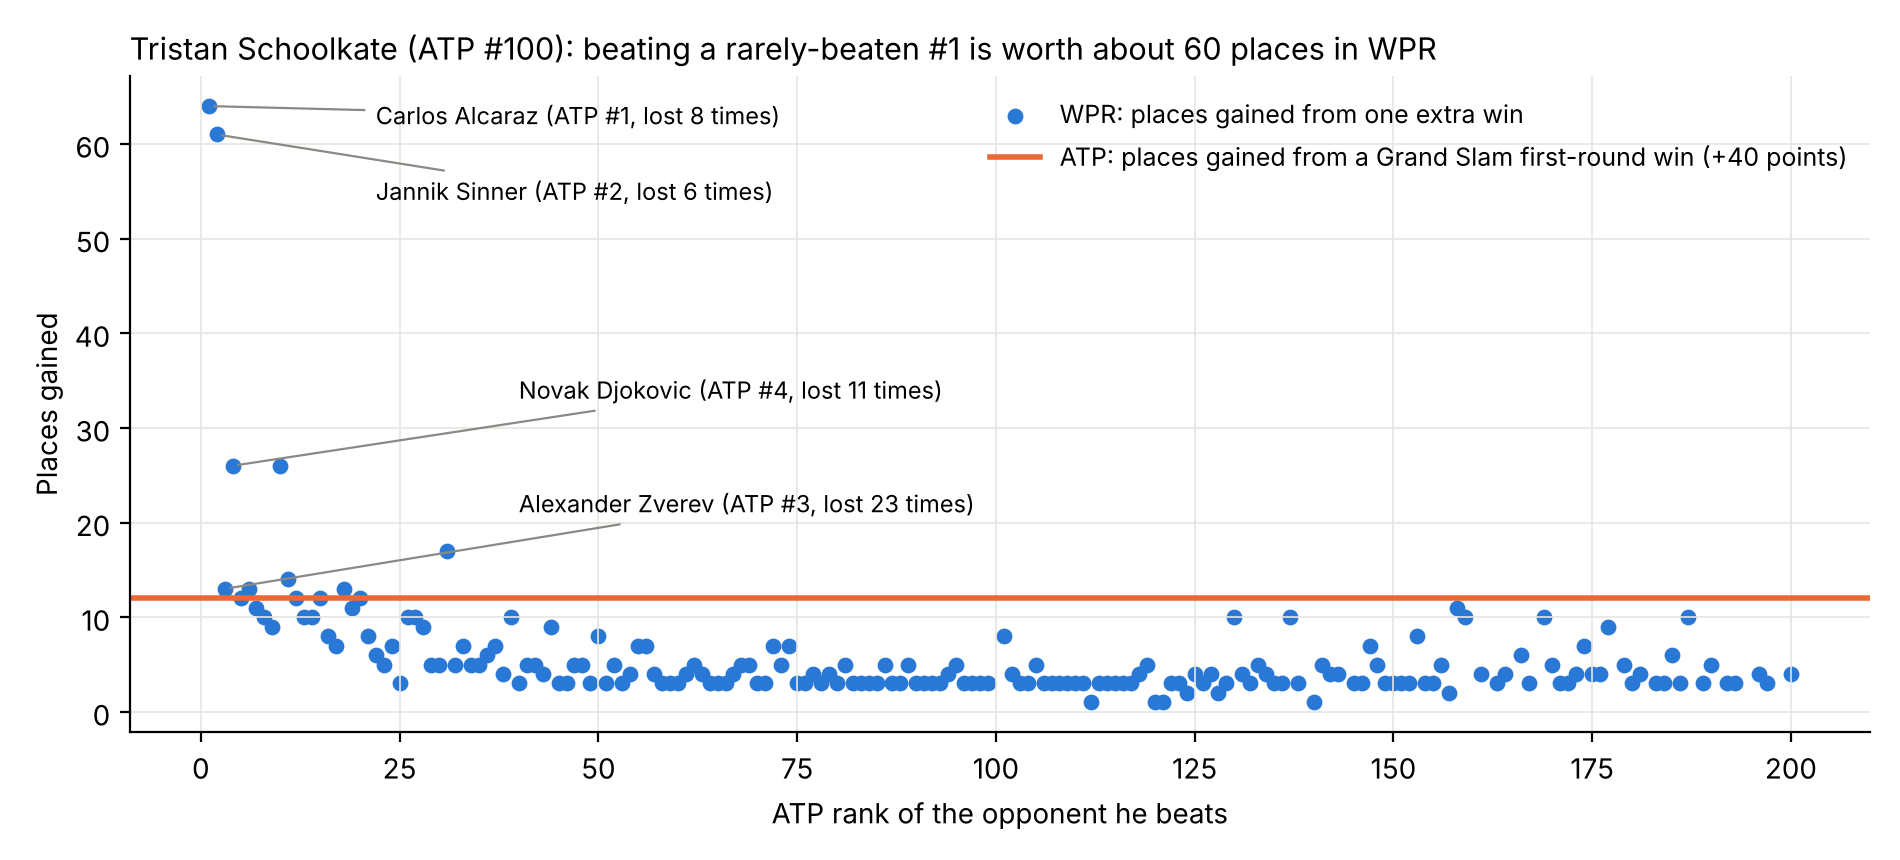
\includegraphics[width=\linewidth]{figures/upset_experiment.png}
\caption{Places gained by the ATP number 100 from one extra win, depending on the opponent (2025 season). Blue: WPR. Orange: ATP ranking (+40 points, the same for every opponent).}
\label{fig:upset}
\end{figure}

\begin{table}[h]
\centering
\caption{One extra win for the ATP number 100 in 2025. The value of a win depends on how rarely the beaten player loses, not on his ATP rank.}
\label{tab:upset}
\small
\begin{tabular}{lrrrr}
\toprule
Opponent & ATP rank & Losses in 2025 & WPR rank after & Places gained \\
\midrule
Carlos Alcaraz & 1 & 8 & 50 & 64 \\
Jannik Sinner & 2 & 6 & 53 & 61 \\
Alexander Zverev & 3 & 23 & 101 & 13 \\
Novak Djokovic & 4 & 11 & 88 & 26 \\
Tommy Paul & 20 & 13 & 102 & 12 \\
Jenson Brooksby & 50 & 15 & 106 & 8 \\
Oliver Crawford & 200 & 1 & 110 & 4 \\
\midrule
\multicolumn{4}{l}{ATP ranking: +40 points (Grand Slam first-round win), any opponent} & 12 \\
\bottomrule
\end{tabular}
\end{table}

The answer to the meeting question is yes, and it holds beyond one case. One win over Alcaraz or Sinner moves the number 100 up about 60 places in WPR, against 12 in the ATP ranking. For all 21 players ranked 90--110 in 2025, the median WPR rank goes from 104 to 45 after beating Alcaraz, but only to 101 after beating the number 200. Repeating the experiment in every season 1990--2025 (that season's number 100 beats that season's number 1), the gain is always positive (at least 7 places, median 39), larger under WPR than under standard PageRank in 30 of 36 seasons, and largest when the number one rarely lost (Roger Federer lost 4--5 matches in 2005 and 2006).

The mechanism is simple. A win is worth the beaten player's WPR score divided by the number of times he lost. This quantity orders the gains almost perfectly (Spearman 0.96), while the opponent's ATP rank does not (0.44). Beating Alexander Zverev, ATP number 3 but beaten 23 times in 2025, is worth less than beating Jack Draper (number 10, beaten 9 times). Losing does not lower the beaten player's own WPR rank in this test (Alcaraz stays first): WPR rewards wins and does not subtract for losses.

\subsection{Who gains and who loses under WPR}
For the ATP top 100 of every season 2010--2025 (1,598 player-seasons) we define a player's \emph{gain} as his position by the ATP ranking minus his position by WPR within the top 100; a positive gain means WPR ranks him higher. Gain increases with the number of tour-level matches (Spearman 0.18) and with wins over top-20 players (0.19), and decreases with the share of matches played at Grand Slams, Masters 1000 and the ATP Finals ($-0.11$). Table~\ref{tab:gain} shows the two clearest patterns.

\begin{table}[h]
\centering
\caption{Mean gain (ATP position minus WPR position, top 100, 2010--2025). Left: by number of tour-level matches. Right: by share of matches at Grand Slams, Masters 1000 and ATP Finals.}
\label{tab:gain}
\small
\begin{tabular}{lrr@{\hspace{2.5em}}lrr}
\toprule
Tour-level matches & Players & Mean gain & Share at big events & Players & Mean gain \\
\midrule
20 or fewer & 274 & $-8.1$ & up to 30\% & 347 & $+1.5$ \\
21--30 & 222 & $+0.8$ & 30--45\% & 613 & $+1.5$ \\
31--40 & 284 & $+2.9$ & 45--60\% & 432 & $-0.9$ \\
41--60 & 613 & $+1.7$ & 60--75\% & 142 & $-4.5$ \\
more than 60 & 205 & $+0.9$ & over 75\% & 48 & $-7.0$ \\
\bottomrule
\end{tabular}
\end{table}

Two features of the ATP ranking explain these patterns. It rewards a single deep run heavily: Valentin Vacherot won the 2025 Shanghai Masters as a qualifier, which is worth 1,000 ATP points, but it adds only 11 tour-level wins to the graph. And it includes points from the Challenger tour, which is not in our tour-level graph, so players who play few tour-level matches lose places under WPR. In 2025 the largest losers were Sebasti\'an B\'aez (ATP 45, no wins over top-20 players, 61\% of matches on clay), Valentin Royer and Terence Atmane (21 and 17 tour-level matches); the largest gainers were Benjamin Bonzi (ATP 94) and Roberto Bautista Agut (ATP 90), who each won fewer than half of their tour-level matches but beat three top-20 players.

\paragraph{Location.} South American players are ranked on average 2.0 places lower by WPR than by the ATP ranking (164 player-seasons; all other players $+0.2$; Mann--Whitney $p = 0.014$). Their seasons are clay-heavy (53\% of matches on clay, against 32\% for Europeans), and many of their matches are at ATP 250 events in South America. An ATP 250 title is worth 250 points everywhere, but the fields are not equally strong everywhere (Table~\ref{tab:region}): the median beaten player at ATP 250 events in South America was ranked 89 at the end of the year, against 63 in Asia and 70 in Europe. The same points therefore come with fewer wins over strong players, and WPR gives less credit. (Tournament locations were entered by hand; this is an association, not a proof of cause.)

\begin{table}[h]
\centering
\caption{ATP 250 matches 2010--2025 by continent of the tournament: median year-end ATP rank of the beaten player.}
\label{tab:region}
\small
\begin{tabular}{lrrrr}
\toprule
Region & Tournaments & Matches & Median rank of beaten player & Share on clay \\
\midrule
Asia & 110 & 3,224 & 63 & 0\% \\
Oceania & 47 & 1,340 & 68 & 0\% \\
Europe & 427 & 12,430 & 70 & 43\% \\
North America & 137 & 4,417 & 85 & 11\% \\
South America & 62 & 1,775 & 89 & 92\% \\
Africa & 16 & 450 & 97 & 86\% \\
\bottomrule
\end{tabular}
\end{table}

\subsection{Across sports and ranking styles}
\label{sec:sports}
Table~\ref{tab:sports} applies the same WPR to sports whose official rankings follow different rules. A draw counts as half a win in each direction. For international football we compare with the full FIFA men's ranking of 18 July 2024 \citep{fifa2024}, the most recent complete list we could access, using all matches between FIFA members from 16 August 2018 (when FIFA adopted its Elo-based method) to 18 July 2024 \citep{intlresults}.

\begin{table}[h]
\centering
\caption{Spearman between WPR (or standard PageRank) and the official ranking, by sport and ranking style. ``Games per pair'' = matches divided by the number of different pairs that met. Tennis: top 100 of the official ranking. Data: \citep{sackmann,wtadata,intlresults,footballdatasets,hoopr,fastrhockey,nflverse,wiki_nhl2526}.}
\label{tab:sports}
\small
\begin{tabularx}{\linewidth}{L l r r r r}
\toprule
Sport (season) & Official ranking style & Games per pair & Pairs met & WPR & Standard \\
\midrule
Men's tennis, ATP (2025) & Tournament points & 1.17 & 5\% & 0.915 & 0.914 \\
Women's tennis, WTA (2025) & Tournament points & 1.15 & 4\% & 0.877 & 0.874 \\
International football, 210 teams (2018--24) & Elo rating (FIFA) & 1.95 & 13\% & 0.947 & 0.955 \\
\quad same, FIFA top 50 & Elo rating (FIFA) & & & 0.771 & 0.653 \\
Premier League (2025--26) & League table & 2.00 & 100\% & 0.956 & 0.799 \\
NBA (2025--26) & League + playoffs & 2.83 & 100\% & 0.962 & 0.876 \\
NHL (2025--26) & League + playoffs & 2.65 & 100\% & 0.875 & 0.815 \\
NFL (2025) & League + playoffs & 1.21 & 45\% & 0.888 & 0.880 \\
\bottomrule
\end{tabularx}
\end{table}

\begin{figure}[h]
\centering
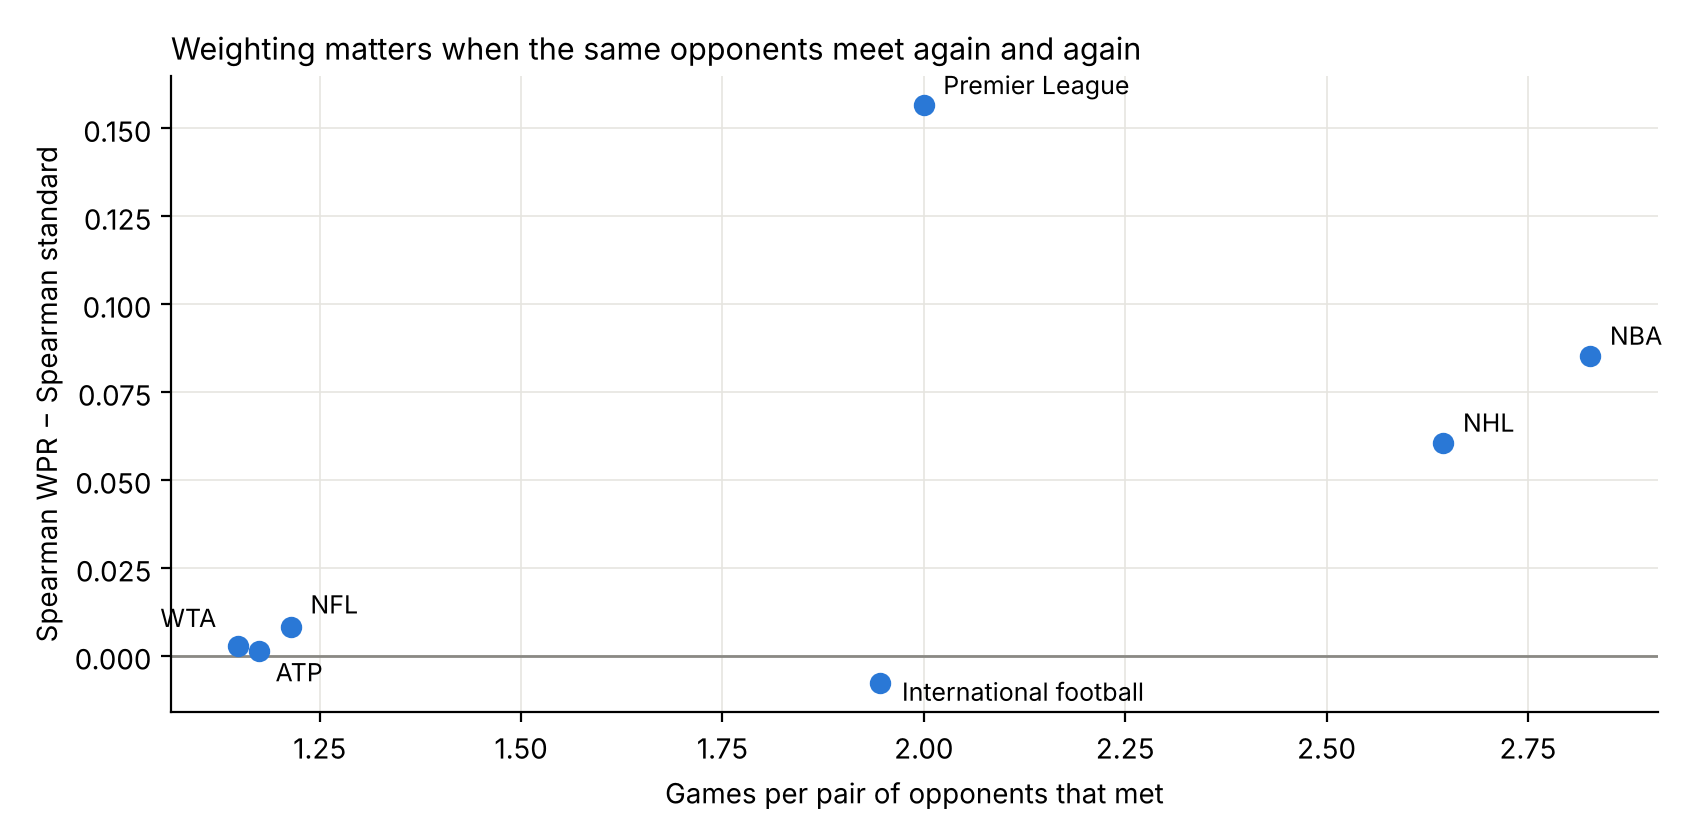
\includegraphics[width=0.82\linewidth]{figures/weighting_gain_by_sport.png}
\caption{Improvement from weighting (Spearman of WPR minus Spearman of standard PageRank) against the number of games per pair of opponents that met.}
\label{fig:sports}
\end{figure}

Two results stand out (Figure~\ref{fig:sports}). First, weighting matters in proportion to how often the same opponents meet: it adds 0.16 in the Premier League, 0.09 in the NBA and 0.06 in the NHL, but almost nothing in tennis and the NFL, where most pairs meet once. International football is the exception at the level of all 210 teams, but among the FIFA top 50 weighting adds 0.12. Second, agreement is lowest where the official ranking uses information that WPR does not have: the COVID freeze of 2020 (ATP 0.70, WTA 0.72), points from the Challenger tour, points for overtime losses in the NHL (WPR counts them as ordinary losses), and the FIFA top 50, in a sport where teams rarely play opponents from other continents (only 13\% of all pairs of teams met). Chess (FIDE Elo) and golf (Official World Golf Ranking) fit the same framework; chess needs an open file of rated classical games, and golf, which is not head-to-head, needs a different graph (for example, each player beats everyone who finished behind him in a tournament). Both are left for future work.

\subsection{Conclusions of this section}
\begin{enumerate}
\item \emph{Can we state that weighted PageRank is better?} Better than standard PageRank at agreeing with official rankings: yes, consistently in tennis (small effect) and strongly in leagues with repeated games. Better than the official ranking at predicting results: no; in men's tennis they are tied and in women's tennis the WTA ranking is slightly better.
\item \emph{Is the high correlation good or bad?} It confirms that the official rankings mostly agree with head-to-head results. The useful information is in where they disagree.
\item \emph{Who gains under WPR?} Players with many wins over strong, rarely beaten opponents. \emph{Who loses?} Players whose points come from one deep run, from Challenger events, or from weaker regional fields.
\item \emph{One upset over the number one} is worth about 60 places in WPR and 12 in the ATP ranking; the value of a win depends on how rarely the beaten player loses.
\end{enumerate}

\bibliographystyle{plainnat}
\bibliography{section}
\end{document}
